\documentclass[12pt, a3paper, portrait]{tikzposter}

\usepackage[student]{Lecture}

\title{Corps purs}
%\author{Overleaf Team}
%\date{\today}
%\institute{Overleaf Institute}


%\usepackage[default,oldstyle,scale=0.95]{opensans}
\usepackage{blindtext}
\usepackage{comment}
\usepackage{multirow}
%\usepackage{subfigure}
%\usepackage{tikzfigure}
%\usepackage{subfig}
%\usepackage{subfloat}
\usetheme{Board}

\settitle{ \centering \vbox{
\@titlegraphic \\[\TP@titlegraphictotitledistance] \centering
\color{titlefgcolor} {\bfseries \Huge \sc \@title \par}
%\vspace*{1em}
%{\huge \@author \par} \vspace*{1em} {\LARGE \@institute}
}}

\definetitlestyle{sampletitle}{
width=500mm, roundedcorners=20, linewidth=2pt, innersep=5pt,
titletotopverticalspace=15mm, titletoblockverticalspace=15mm
}{
\begin{scope}[line width=\titlelinewidth, rounded corners=\titleroundedcorners]
\draw[color=blocktitlebgcolor, fill=titlebgcolor]
(\titleposleft,\titleposbottom) rectangle (\titleposright,\titlepostop);
\end{scope}
}

%\newcolumntype{C}[1]{>{\centering\let\newline\\\arraybackslash\hspace{0pt}}m{#1}}  
\begin{document}
\usetitlestyle{sampletitle}
\maketitle
%\@title
%\end{figure}
\begin{columns}
\column{0.25}
\block{Définitions}{
\textbf{Corps purs} : Corps constitués d'entités moléculaires identiques.
\begin{itemize}
\item \textbf{corps simples} : entité moléculaire constituée d'atomes de même natures (c.-à-d. constituée du même élément chimique).
\item \textbf{corps composés} : entité moléculaire constituée d'atomes de natures différents.
\end{itemize}
\textbf{Mélanges} : Association de plusieurs entités moléculaires différentes formant une ou plusieurs phases.
\begin{itemize}
\item \textbf{homogènes}  : une phase ;
\item \textbf{hétérogènes} : plusieurs phases distinguables à l'{\oe}il nu ou au microscope ;
\item \textbf{colloïdales} : plusieurs phases qui semblent homogènes à l'{\oe}il nu, mais qui sont observables au microscope.
\end{itemize}
}

\column{0.25}
\block{Carte heuristique}{\centering 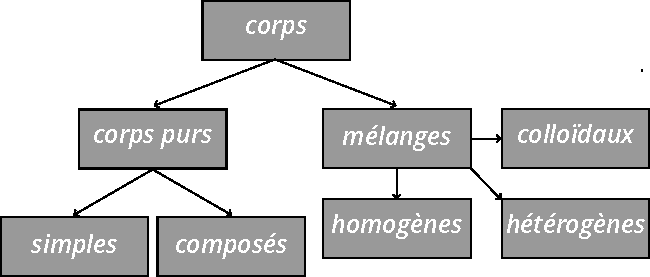
\includegraphics[width=0.9\colwidth]{../CP.pdf}}


\column{0.5}
\block{Exemples}{
\begin{minipage}[t][.12\textwidth][c]{0.3\colwidth}
	\centering
   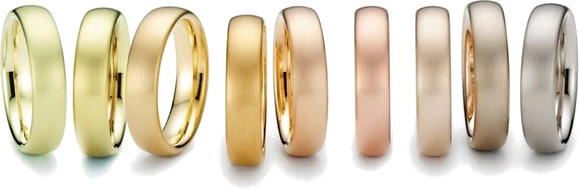
\includegraphics[width=\textwidth]{../figures/Fig15a}
   \captionof{figure}{Mélange homogène : \'{E}volution de la couleur du mélange or-argent-cuivre en fonction des fractions massiques en chacun des composés.}
\end{minipage}\hfill\begin{minipage}[t][.12\textwidth][c]{0.3\colwidth}
   \centering
   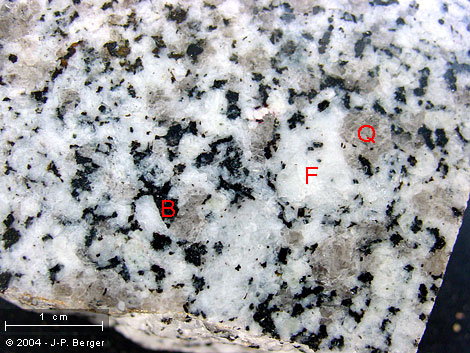
\includegraphics[width=0.9\textwidth]{../figures/Fig16a}
   \captionof{figure}{Mélange Hétérogène : Granite constitué de trois cristaux non miscibles la biotite (un mica noir) {\color{red} \textbf{(B)}}, le feldspath {\color{red} \textbf{(F)}} et le quartz {\color{red} \textbf{(Q)}}}
\end{minipage}\hfill\begin{minipage}[t][.12\textwidth][c]{0.3\colwidth}
   \centering
   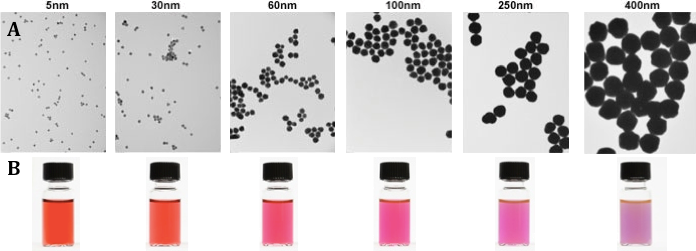
\includegraphics[width=\textwidth]{../figures/Fig17}
   \captionof{figure}{Mélange colloïdal : Les nanoparticules d'or dans l'eau, un mélange en apparence homogène, mais hétérogène à l'échelle microscopique. La taille des particules influence la couleur de la solution (absorption de lumière dépend de la taille des particules).}
\end{minipage}
%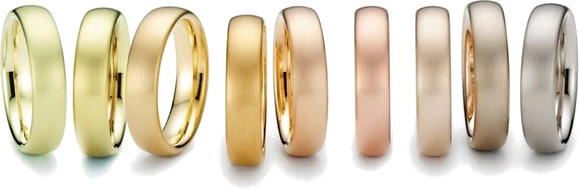
\includegraphics[height=1.0\colheight]{../figures/Fig15a}
%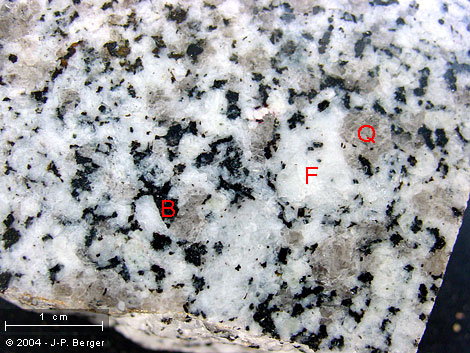
\includegraphics[height=1.0\colheight]{../figures/Fig16a}
%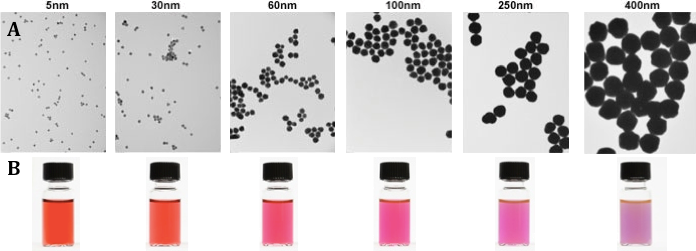
\includegraphics[height=1.0\colheight]{../figures/Fig17}
}
%\begin{subfigure}{0.5\colwidth}
%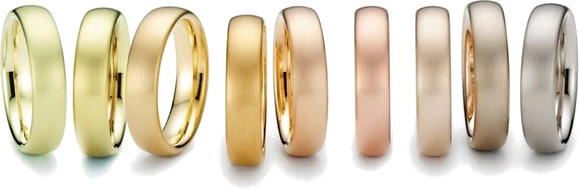
\includegraphics{../figures/Fig15a}
%\end{subfigure}\begin{subfigure}{0.5\colwidth}
%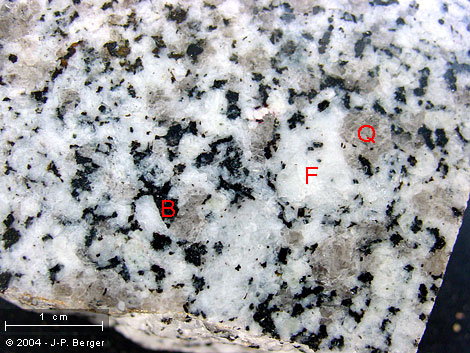
\includegraphics[width=0.3\colwidth]{../figures/Fig16a}
%\end{subfigure}
%\begin{tikzfigure}
%\subfloat[]{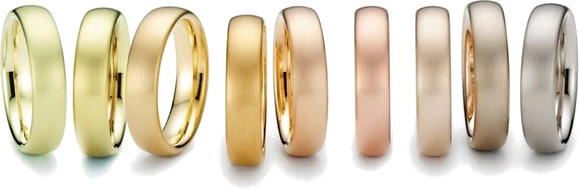
\includegraphics[width=0.3\colwidth]{../figures/Fig15a}}
%\subfloat[]{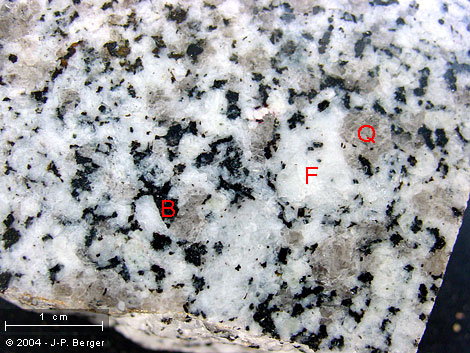
\includegraphics[width=0.3\colwidth]{../figures/Fig16a}}%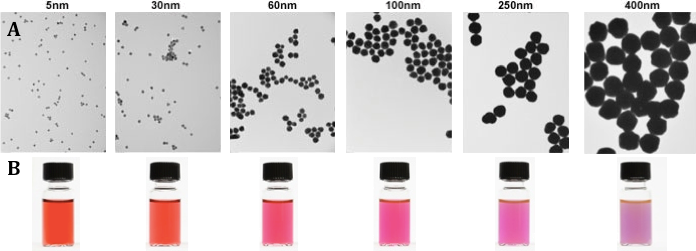
\includegraphics[width=0.3\colwidth]{../figures/Fig17}
%\end{tikzfigure}
%}

\end{columns}

\begin{columns}
	\column{0.25}
\block{Etat solide : définitions}{
\textbf{Etat cristallin} Microscopiquement, un ensemble d'atome, appelé motif, occupe des positions périodiques dans l'espace appelées \og n{\oe}uds \fg{}. Un ensemble de n{\oe}uds forment un réseau.

La stabilité d'une forme cristalline/ un état cristallin à l'équilibre thermodynamiques dépend des conditions de pression et température. On utilise deux termes de vocabulaires : 
\begin{itemize}
\item \textbf{Allotropie} : Faculté de certains corps simples d'exister sous plusieurs formes cristallines ou moléculaires différentes.

\item \textbf{Polymorphisme} : Faculté de certains corps composés d'exister sous plusieurs formes cristallines ou moléculaires différentes .
\end{itemize}

\textbf{État vitreux} Solides vitreux possèdent les mêmes caractéristiques qu'un solide cristallin : rigidité, résistance à la déformation mais, leur structure microscopique est analogue à un liquide.}

\column{0.25}
\block{Carte heuristique}{\centering 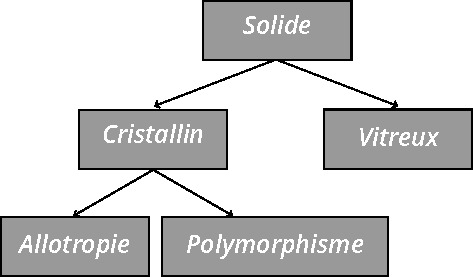
\includegraphics[width=0.68\colwidth]{../CP2.pdf}}

\column{0.5}
\block{Exemples}{
\begin{center}
\begin{minipage}[t][.07\textwidth][c]{0.55\colwidth}
\centering
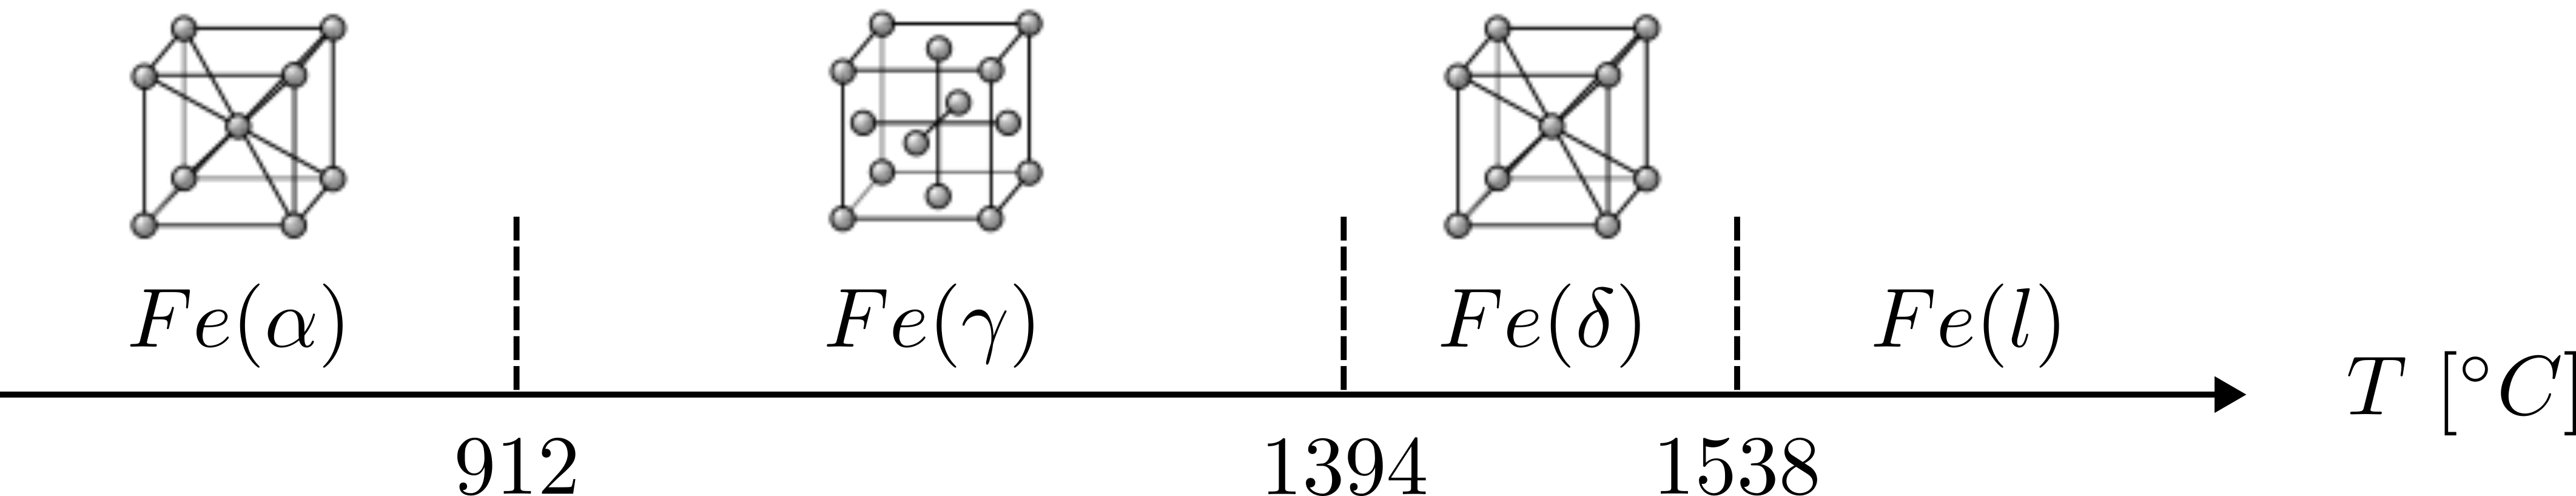
\includegraphics[width=0.9\textwidth]{../figures/Fig18}
\captionof{figure}{Variétés allotropiques du fer à pression ambiante}
\end{minipage}\begin{minipage}[t][.07\textwidth][c]{0.4\colwidth}
\centering
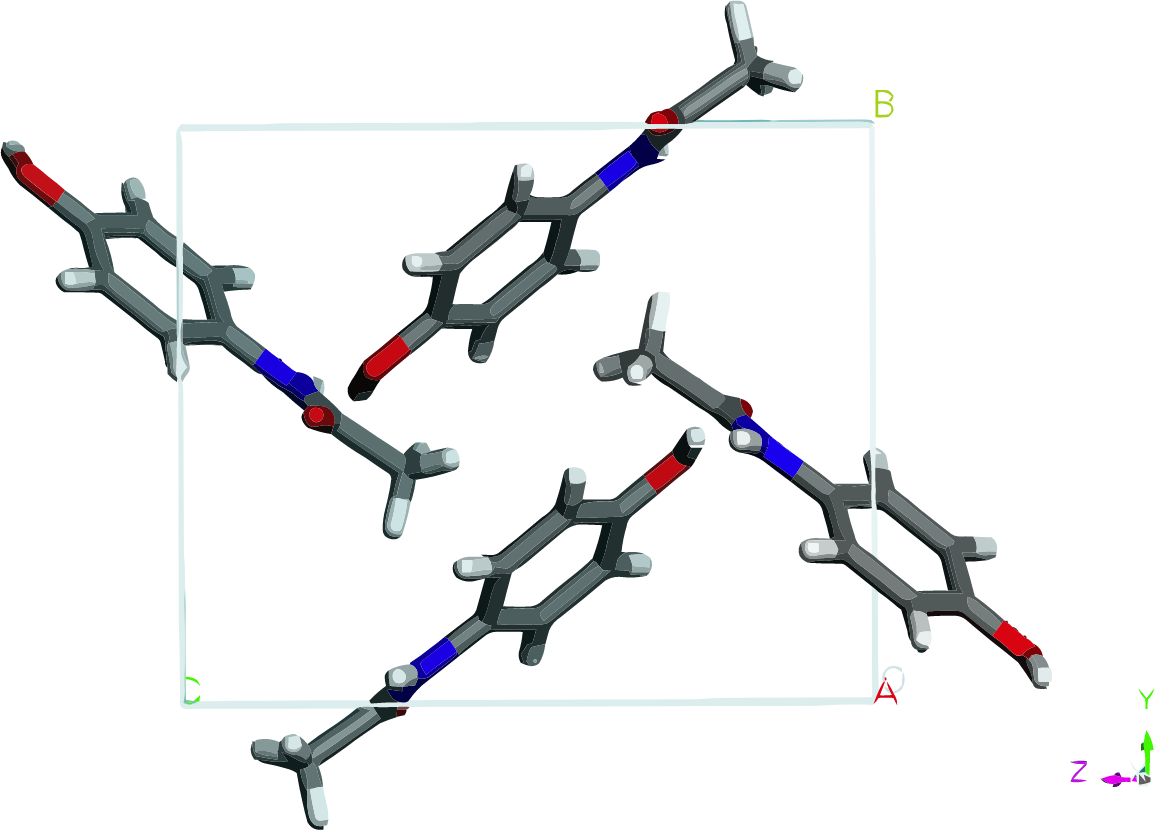
\includegraphics[width=0.5\textwidth]{../figures/Fig01a}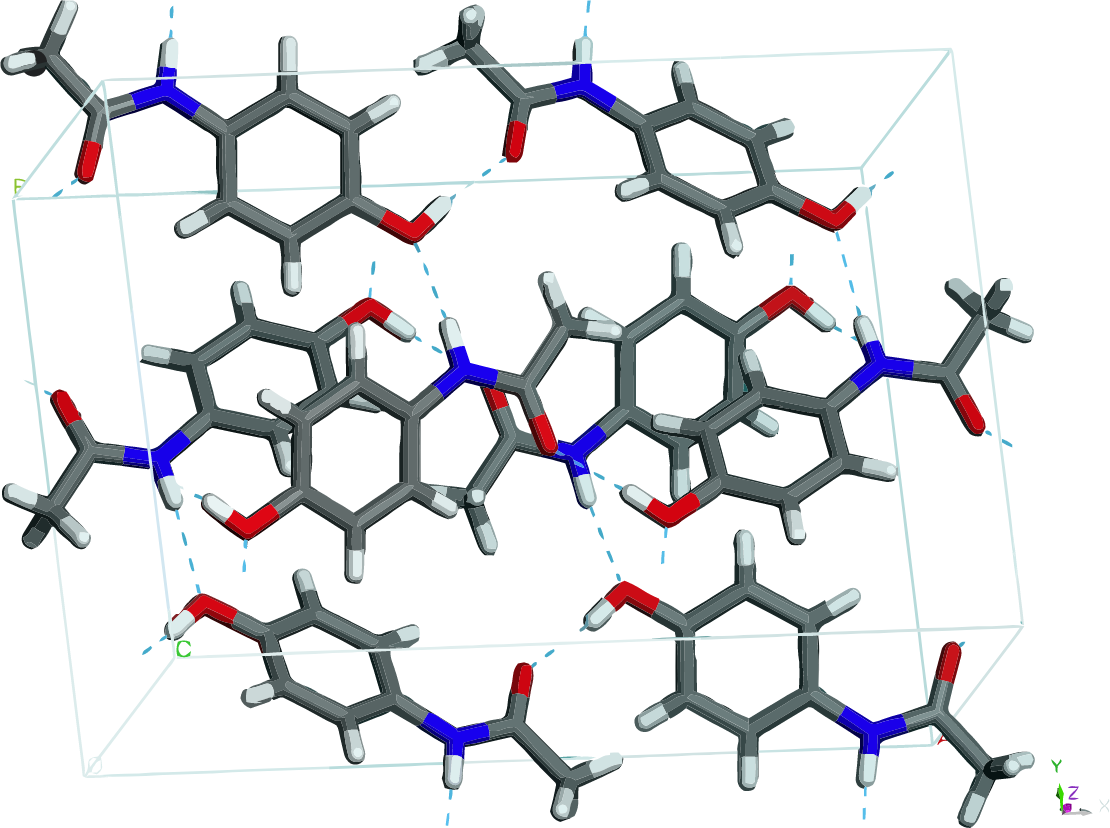
\includegraphics[width=0.5\textwidth]{../figures/Fig01b}
\captionof{figure}{Polymorphes du paracétamol monoclinique (gauche) \& orthorhombique (droite). [La maille monoclinique (resp. orthorhombique) contient 4 molécules (resp. 8 molécules). La forme $n^\circ 1$ est celle présente dans les comprimés pharmaceutiques]}
\label{fig:Fe}
\end{minipage}
\end{center}
}

\end{columns}

\begin{columns}
    \column{0.25}
    \block{\'{E}tats physiques de la matière}
    {\textbf{Définitions} \\
    \begin{center}
		\begin{tabular}{C{4cm}C{4cm}C{4cm}}
		\toprule
		Gaz & Liquide & Solide \\
		\midrule 
		Occupe tout le volume $V$ qui lui est offert & Occupe leur volume propre mais prennent la forme du récipient & Occupe leur volume propre, et garde leur forme \\\bottomrule
	\end{tabular}
	\end{center}

    \textbf{Transitions de phases} Transitions du premier ordre, c'est-à-dire que ce sont les dérivées premières de $G$ qui sont discontinues.\\
        \begin{tikzfigure}
            
\includegraphics[width=0.15\textwidth]{../figures/Fig04}
        \end{tikzfigure}
    }
    \column{0.5}
    \block{Propriétés d'un corps pur}{
	\textbf{Volume molaire} Le volume molaire d'un corps pur, dans une phase donnée, indique le volume occupé par une mole du corps pur à température et pression fixée. On le définit par :  
	\begin{align*}
	V_m^\star (T, P) = \frac{V(T,P,n)}{n}
	\end{align*}

	Tendance : \begin{align*}
	V_m^\star (g) > V_m^\star (l) > V_m^\star (s)
	\end{align*}

	\textbf{Masse volumique} La masse volumique d'un corps pur, dans une phase donnée, indique la masse correspondant à un mètre cube à température et pression fixée. On le définit par :
	\begin{align*}
	\rho^\star (T, P) = \frac{m(n)}{V(T, P, n)}
	\end{align*}

	Tendance : \begin{align*}
	\rho^\star (s) > \rho^\star (l) > \rho^\star (g)
	\end{align*}
	
	\textbf{Entropie molaire} L'entropie molaire d'un corps pur, dans une phase donnée, indique l'entropie d'une mole du corps pur à température et pression fixée.
	\begin{align*}
	S_m^\star (T, P) = \frac{S(n)}{n}
	\end{align*}	
	Tendance : \begin{align*}
	S_m^\star (g) > S_m^\star (l) > S_m^\star (s)
	\end{align*}
    }
    
    \column{0.25}
    \block{Exemples \& Exceptions}{
    \begin{center}
    \begin{tabular}{cccc}
\toprule
\'{E}lement \& Phase & \ce{CO2(g)} & \ce{CO2(l)} & \ce{CO2(s)} \\
\midrule
$V_m^\star ~ [\si{\deci\meter\cubed\per\mole}]$ & $22.26$ & $40 \cdot 10^{-3}$ & $28 \cdot 10^{-3}$ \\
\midrule
\'{E}lement \& Phase & \ce{H2O(g)} & \ce{H2O(l)} & \ce{H2O(s)} \\
\midrule
$V_m^\star ~ [\si{\deci\meter\cubed\per\mole}]$ & $-$ & $18 \cdot 10^{-3}$ & $19.63 \cdot 10^{-3}$ \\
\midrule
\'{E}lement \& Phase & \ce{C(graphite)} & \ce{C(diamant)} & - \\
\midrule
$V_m^\star ~ [\si{\deci\meter\cubed\per\mole}]$ & $5.38 \cdot 10^{-3}$ & $3.42 \cdot 10^{-3}$ & $-$ \\
\bottomrule
\end{tabular}\end{center}
Il existe des exceptions comme \ce{H2O}, \ce{Bi} et \ce{Ge} où l'inégalité s'écrit comme :
\begin{align*}
V_m^\star (g) \gg V_m^\star (s) > V_m^\star (l)
\end{align*}}
\end{columns}

\begin{columns}
    \column{0.25}
    \block{Représentations des états physiques d'un système fermé}{
    Représentation des courbes de transitions de phases dans un diagramme $(P,T,V)$ et projections utilisables par le chimiste.
    
\includegraphics[width=0.9\colwidth]{../figures/Fig09}}
    \column{0.5}
    \block{Interprétation de la stabilité des phases - diagramme $(T,P)$}{Diagramme de phase pression-température avec phases solide, liquide, vapeur et supercritique dans le cas de \ce{H2O} et \ce{CO2}.\\
 	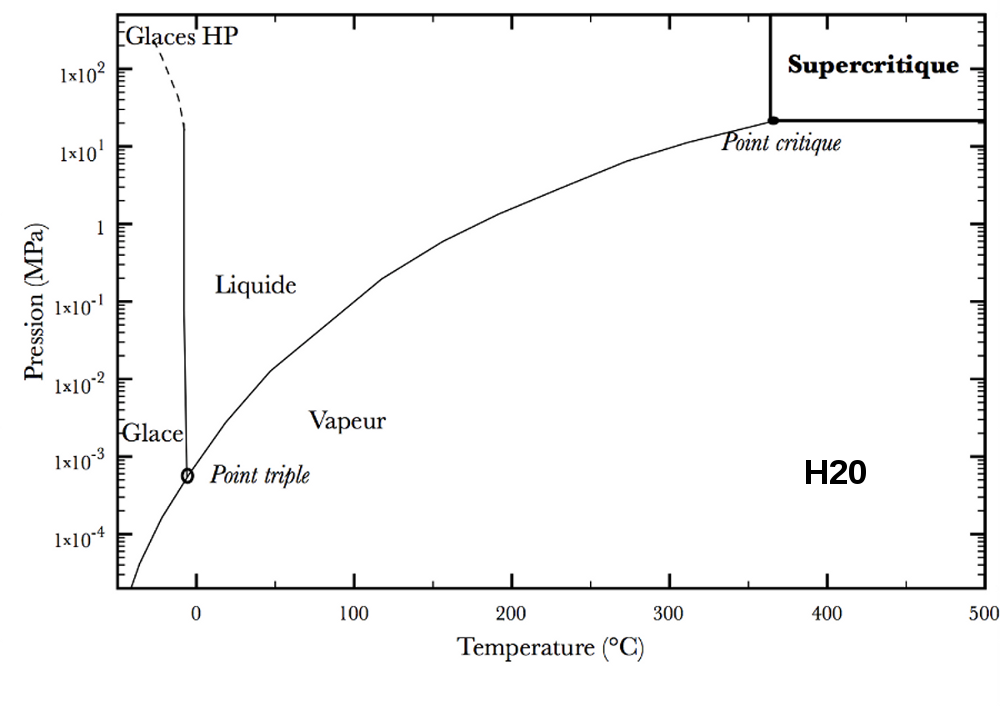
\includegraphics[width=0.40\colwidth]{../figures/Fig07a}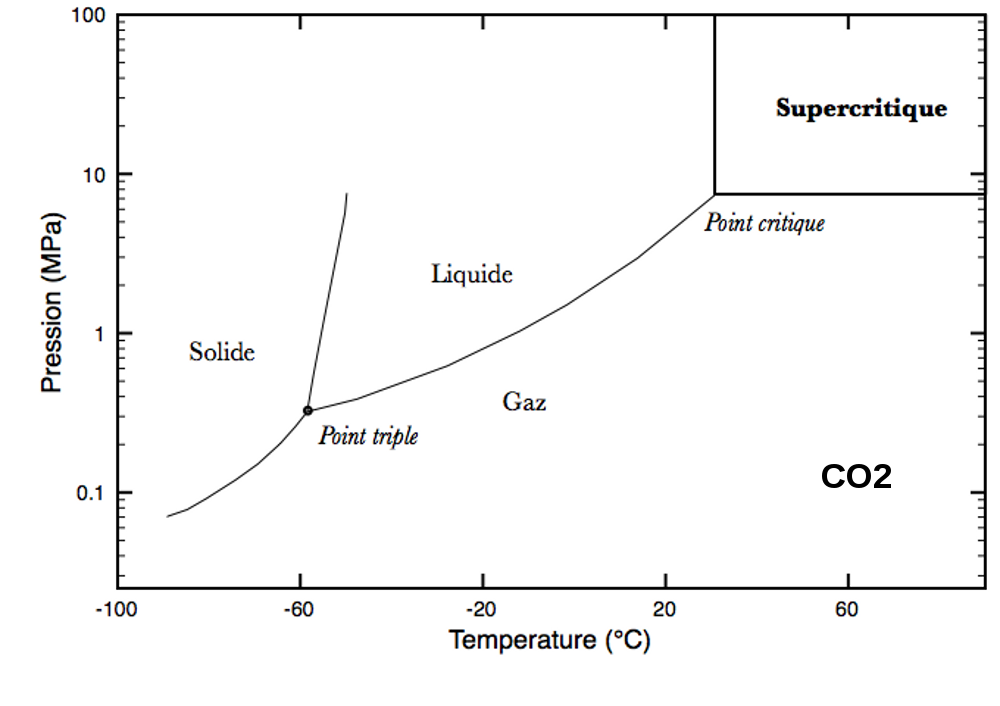
\includegraphics[width=0.40\colwidth]{../figures/Fig07b}   

La position des phases dépend des propriétés de la phase corps pur. Considérons deux phases $\alpha$ et $\beta$ d'un même corps pur : 
\begin{center}
\begin{tabular}{|C{5cm}|C{5cm}|C{5cm}|}
\hline
& $S_{m, \alpha} > S_{m, \beta}$ & $S_{m, \alpha} < S_{m, \beta}$ \\
\hline
 & $\alpha$ Phase HP/HT & $\alpha$ Phase HP/BT  \\
$V_{m, \alpha} < V_{m, \beta}$ & 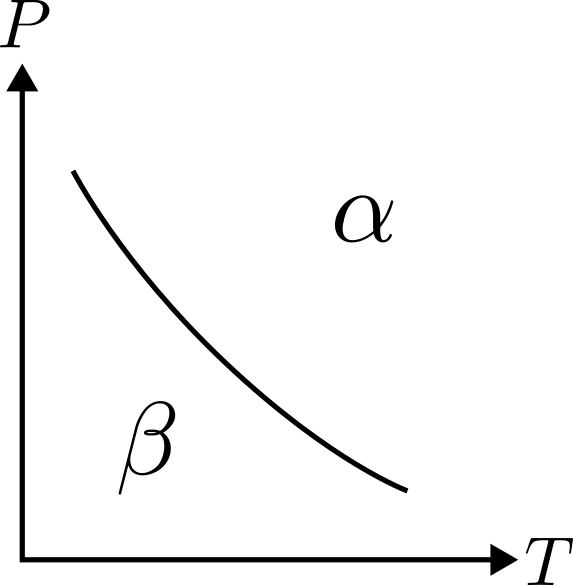
\includegraphics[width=2.9cm]{../figures/Fig24a} & 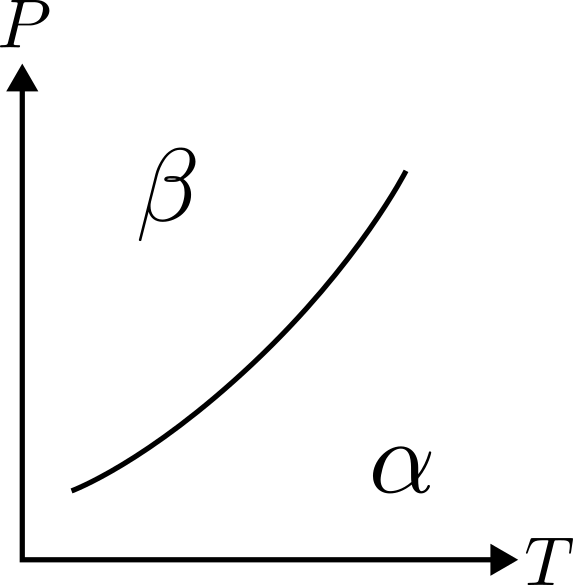
\includegraphics[width=2.9cm]{../figures/Fig24b} \\
\hline
  & $\alpha$ Phase BP/HT   & $\alpha$ Phase BP/BT  \\
$V_{m, \alpha} > V_{m, \beta}$ & 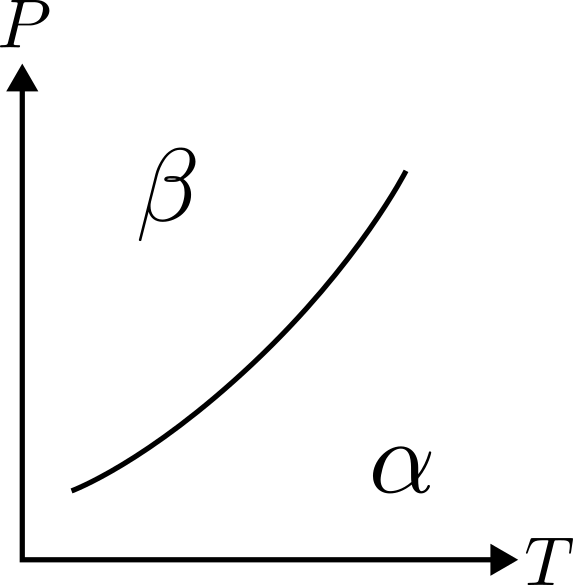
\includegraphics[width=2.9cm]{../figures/Fig24c} & 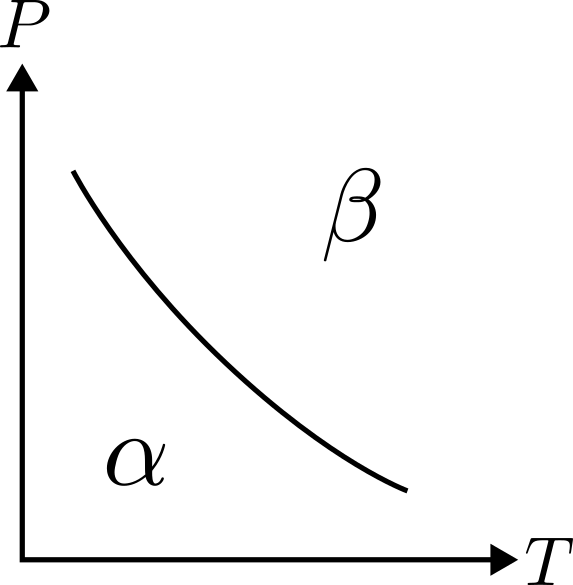
\includegraphics[width=2.9cm]{../figures/Fig24d} \\
\hline
\end{tabular} 
\end{center}
  	
}    

    \column{0.25}
	\block{Diagramme de Clapeyron $(V, T)$ ou $(V, P)$}{Diagramme de Clapeyron $(V, P)$ typique de la majorité des fluides corps purs. [\textbf{S} : solide, \textbf{L} : liquide, \textbf{G} : gaz, \textbf{C} : point critique]
	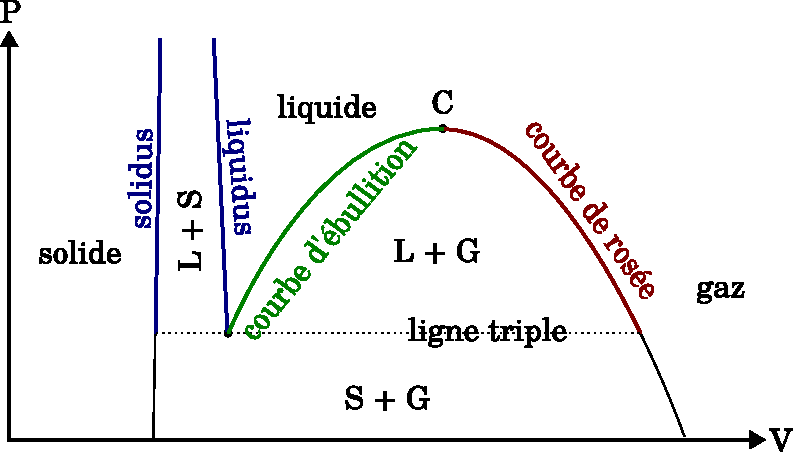
\includegraphics[width=0.9\colwidth]{../figures/Fig19}	

	\begin{itemize}
\item les lignes associées aux transitions solide-liquide :
\begin{enumerate}
\item \textbf{solidus} : ligne dans un diagramme de phase indiquant l'apparition de la première goutte de liquide dans un équilibre liquide-solide ;
\item \textbf{liquidus} : ligne dans un diagramme de phase indiquant l'apparition du premier cristal dans un équilibre liquide-solide ;
\end{enumerate}
\item les lignes associées aux transitions liquide-gaz :
\begin{enumerate}
\item \textbf{courbe d'ébullition} (ou de bulle) : ligne dans un diagramme de phase indiquant l'apparition de la première bulle de gaz dans un équilibre liquide-gaz ;
\item \textbf{courbe de rosée} : ligne dans un diagramme de phase indiquant l'apparition de la première goutte de liquide dans un équilibre liquide-gaz.
\end{enumerate}
	\end{itemize}}

    \column{0.6}
    \block{Something else}{Here, \blindtext \vspace{4cm}}
    \note[
        targetoffsetx=-9cm, 
        targetoffsety=-6.5cm, 
        width=0.5\linewidth
        ]
        {e-mail \texttt{welcome@overleaf.com}}
\end{columns}

\begin{columns}

\column{0.25}

\block{Echauffement d'un corps}{
Les coefficients calorifiques, aussi appelés capacités calorifiques, sont des grandeurs qui permettent de décrire l'évolution de l'énergie du système lors d'une élévation de \SI{1}{\kelvin} de sa température. En général, on regarde cette évolution à volume constant et à pression constante : 
\begin{align*}
C_V = \left( \frac{\partial U}{\partial T} \right)_V \quad  C_p = \left( \frac{\partial H}{\partial T} \right)_P
\end{align*}

Les valeurs tabulées de capacité thermiques le sont généralement de manière intensive en ramenant au nombre de moles ou à la masse du système

\begin{align*}
C_V ~ [\si{\joule\per\kelvin}] &= n ~ [\si{\mole}] \cdot C_{V,m}  ~ [\si{\joule\per\kelvin\per\mole}] = m ~ [\si{\kilo\gram}] \cdot c_V ~ [\si{\joule\per\kelvin\per\kilo\gram}] \\
C_P ~ [\si{\joule\per\kelvin}] &= n ~ [\si{\mole}] \cdot C_{P,m}  ~ [\si{\joule\per\kelvin\per\mole}] = m ~ [\si{\kilo\gram}] \cdot c_P ~ [\si{\joule\per\kelvin\per\kilo\gram}]
\end{align*}

Les capacités thermiques sont liées à la variation en température de l'entropie : 
\begin{align*}
\frac{C_V}{T} = \left( \frac{\partial S}{\partial T} \right)_V \quad  \frac{C_p}{T} = \left( \frac{\partial S}{\partial T} \right)_P
\end{align*}


En intégrant à pression constante, on trouve que :
\begin{align*}
H(T) = H(T_0) + \int_{T_0}^T C_P (T') dT' \quad S(T) = S(T_0) + \int_{T_0}^T \frac{C_P (T')}{T'} dT'
\end{align*}

Représentation de l'évolution de plusieurs grandeurs thermodynamique avec la température lors de l'échauffement d'un solide à pression constante
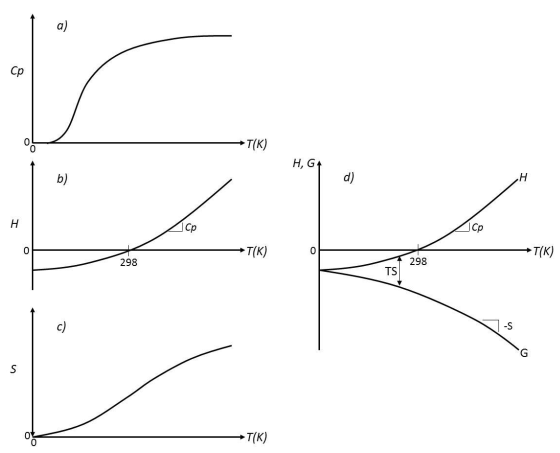
\includegraphics[width=0.9\colwidth]{../figures/Fig14}
%\begin{center}
%\begin{minipage}{0.6\textwidth}
%
\includegraphics[width=\textwidth]{figures/Fig14}
%\end{minipage} \begin{minipage}{0.35\textwidth}
%\captionof{figure}{Représentation de l'évolution de plusieurs grandeurs thermodynamique avec la température lors de l'échauffement d'un solide à pression constante.}
%\end{minipage}
%\end{center}

On peut alors en déduire l'évolution de $G$ à partir de sa définition :
\begin{align*}
G(T) = H(T) - T S(T)
\end{align*}
}



\column{0.5}

\block{Transitions de phases isobares et isothermes}{
\textbf{Hypothèse} : le système est à l'équilibre thermique et mécanique, c'est-à-dire que toutes les phases qui le constituent sont à la même pression et à la même température, et est régi par l'équilibre : 
\begin{align*}
\ce{X ( \alpha ) = X (\beta)} 
\end{align*}

\textbf{Expression de l'enthalpie libre molaire en présence de deux phases $\alpha$ et $\beta$ :}
\begin{align*}
G_m (T, P, x) = \left( \mu_\beta (T, P) - \mu_\alpha (T, P) \right) x + \mu_\alpha (T, P)
\end{align*}
\textbf{Cas de figures :}
\begin{center}
\begin{minipage}[t][.1\textwidth][c]{0.3\colwidth}
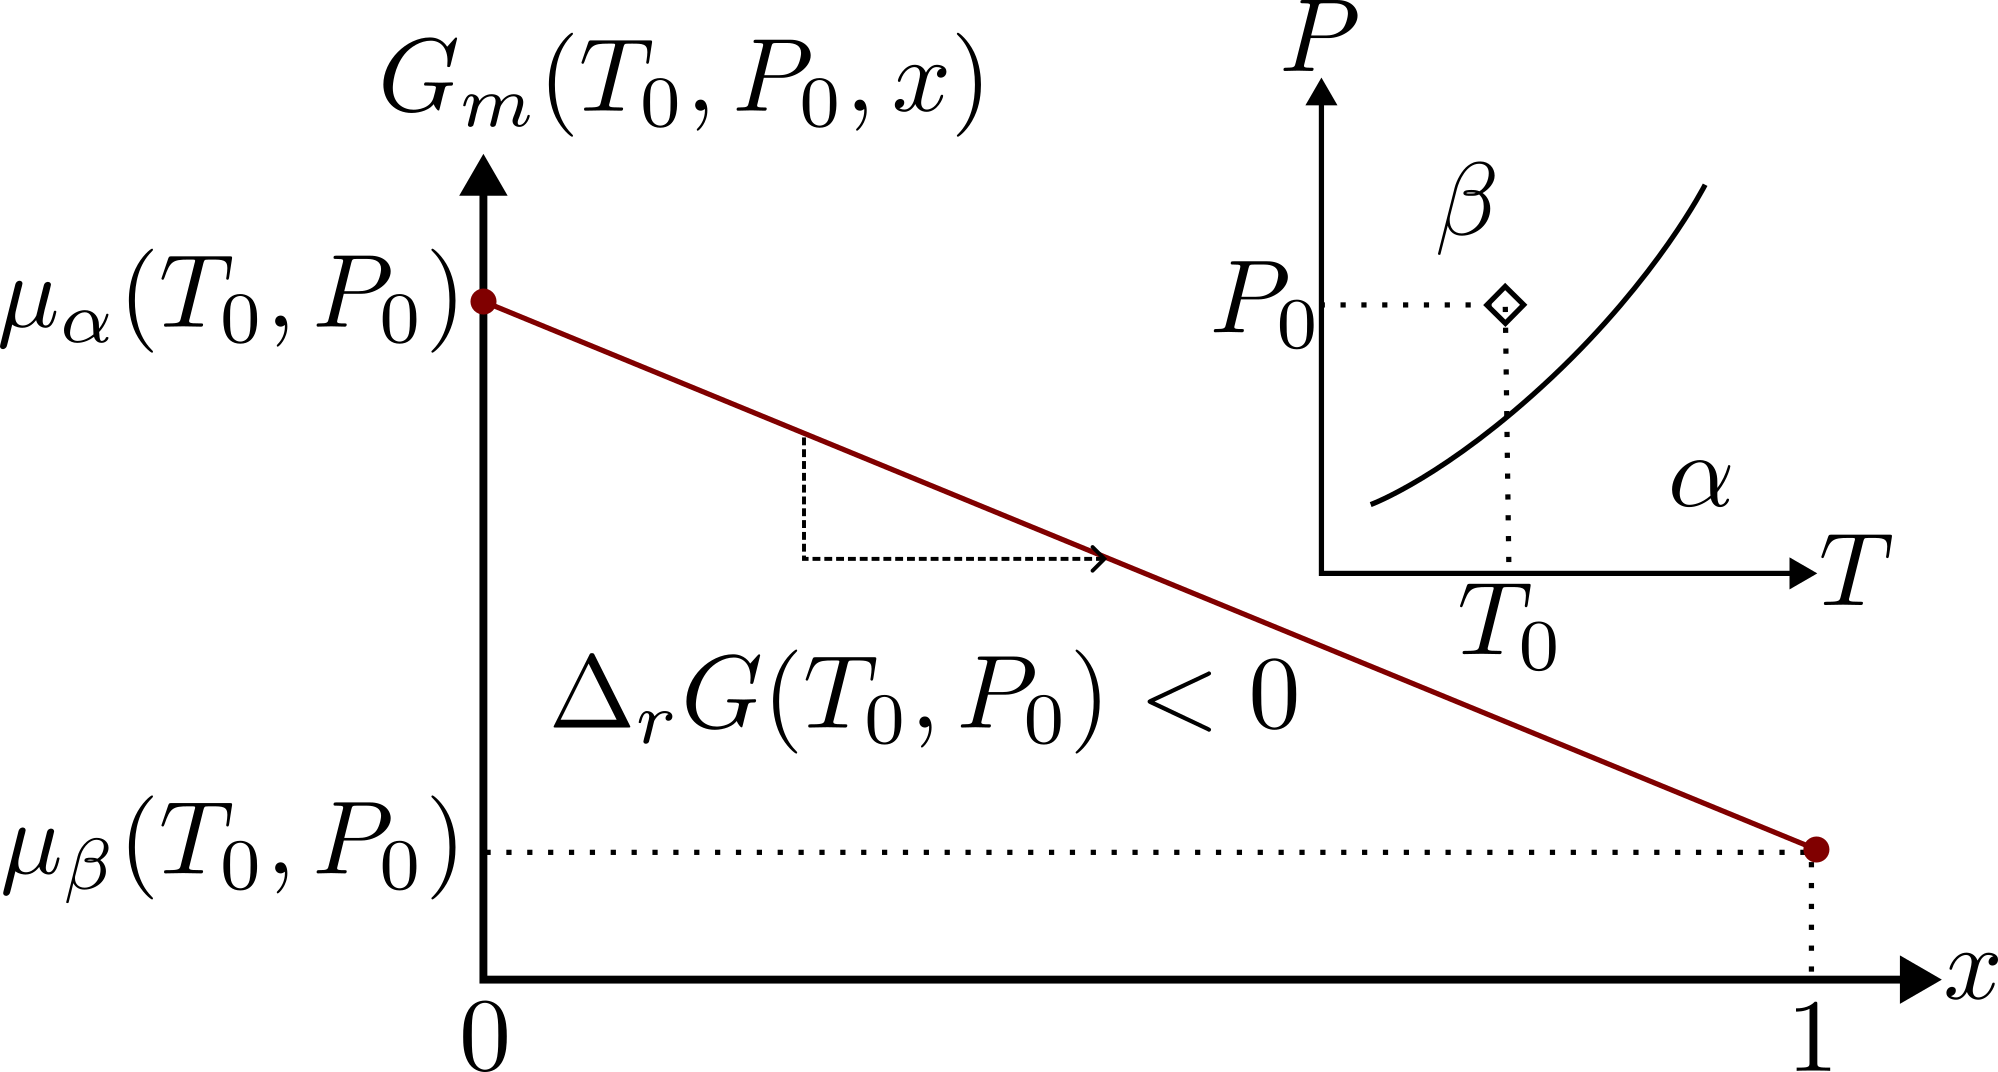
\includegraphics[width=0.25\colwidth]{../figures/Fig22a}
\captionof{figure}{Allure de $G$ en fonction de la fraction $x$ en phase $\beta$ dans le cas où la phase $\beta$ est la plus stable. Position correspondante dans le diagramme $(P,T)$}
\end{minipage}\begin{minipage}[t][.1\textwidth][c]{0.3\colwidth}
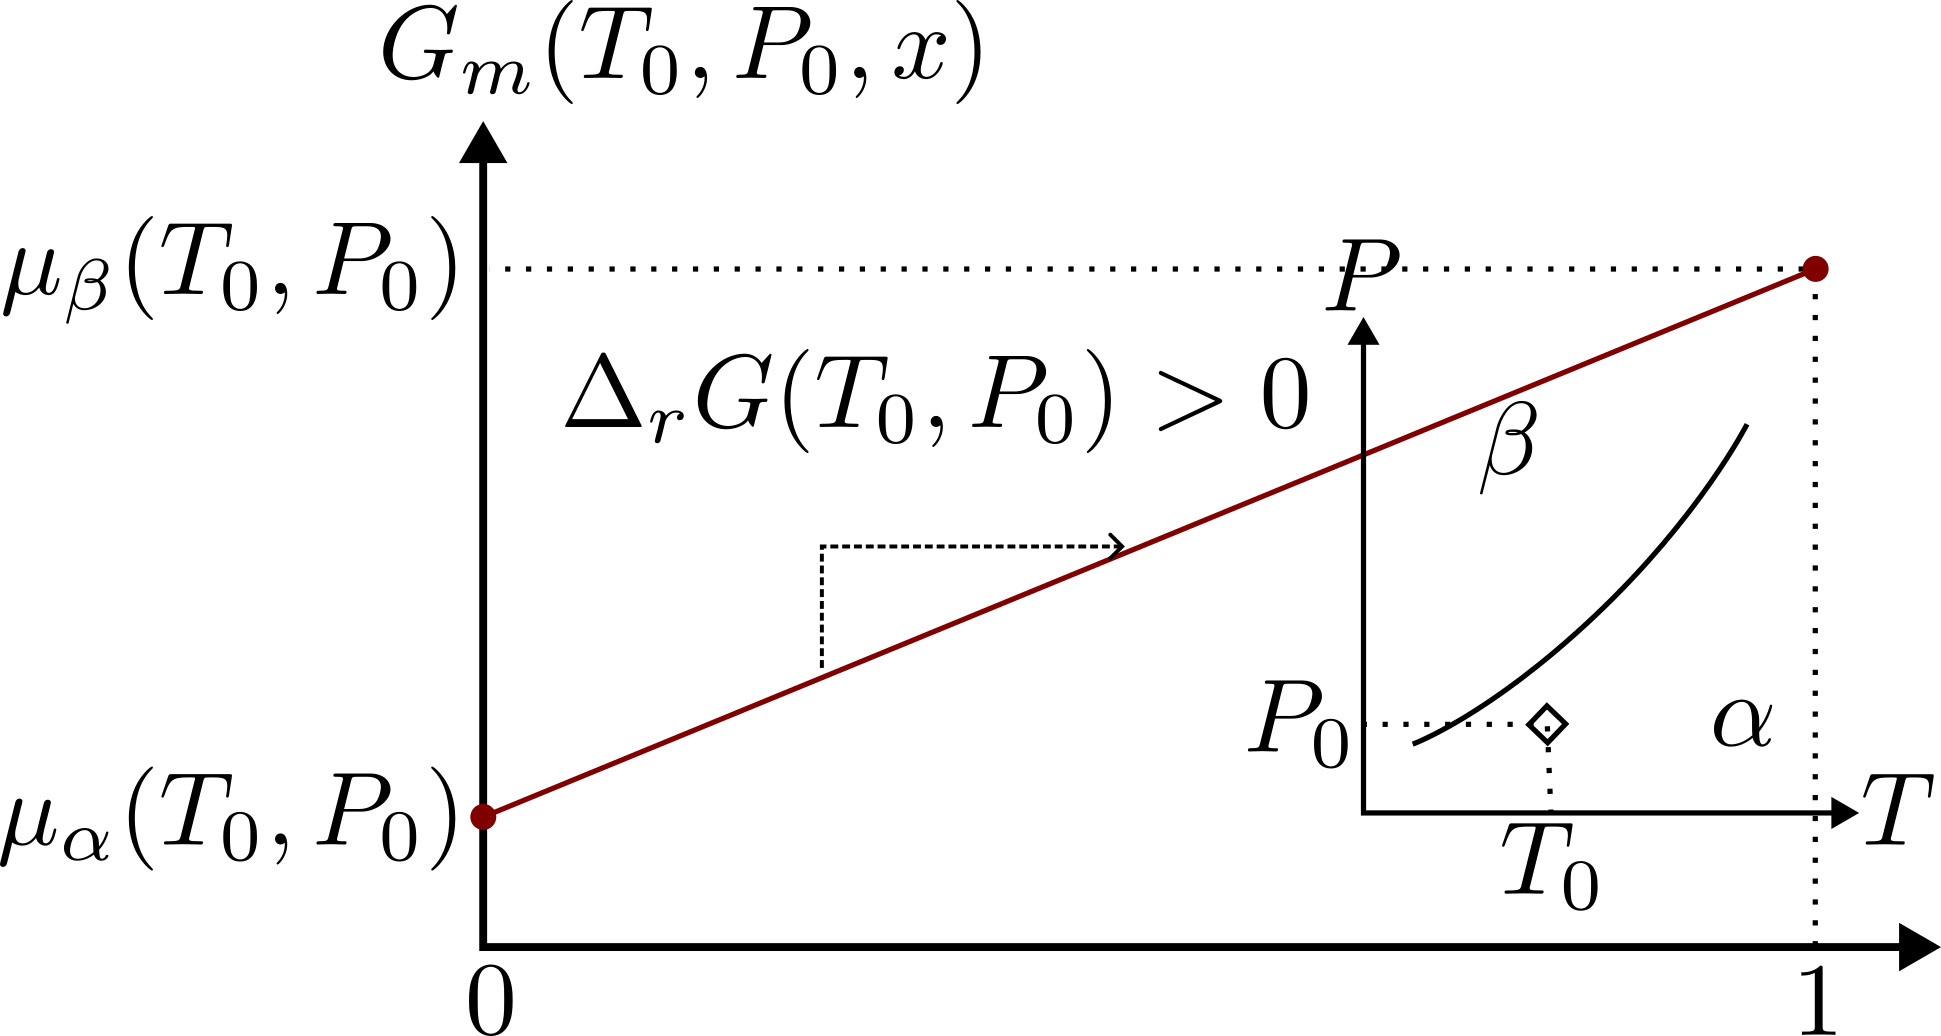
\includegraphics[width=0.25\colwidth]{../figures/Fig22b}
\captionof{figure}{Allure de $G$ en fonction de la fraction $x$ en phase $\beta$ dans le cas où la phase $\alpha$ est la plus stable. Position correspondante dans le diagramme $(P,T)$}
\end{minipage}\begin{minipage}[t][.1\textwidth][c]{0.3\colwidth}
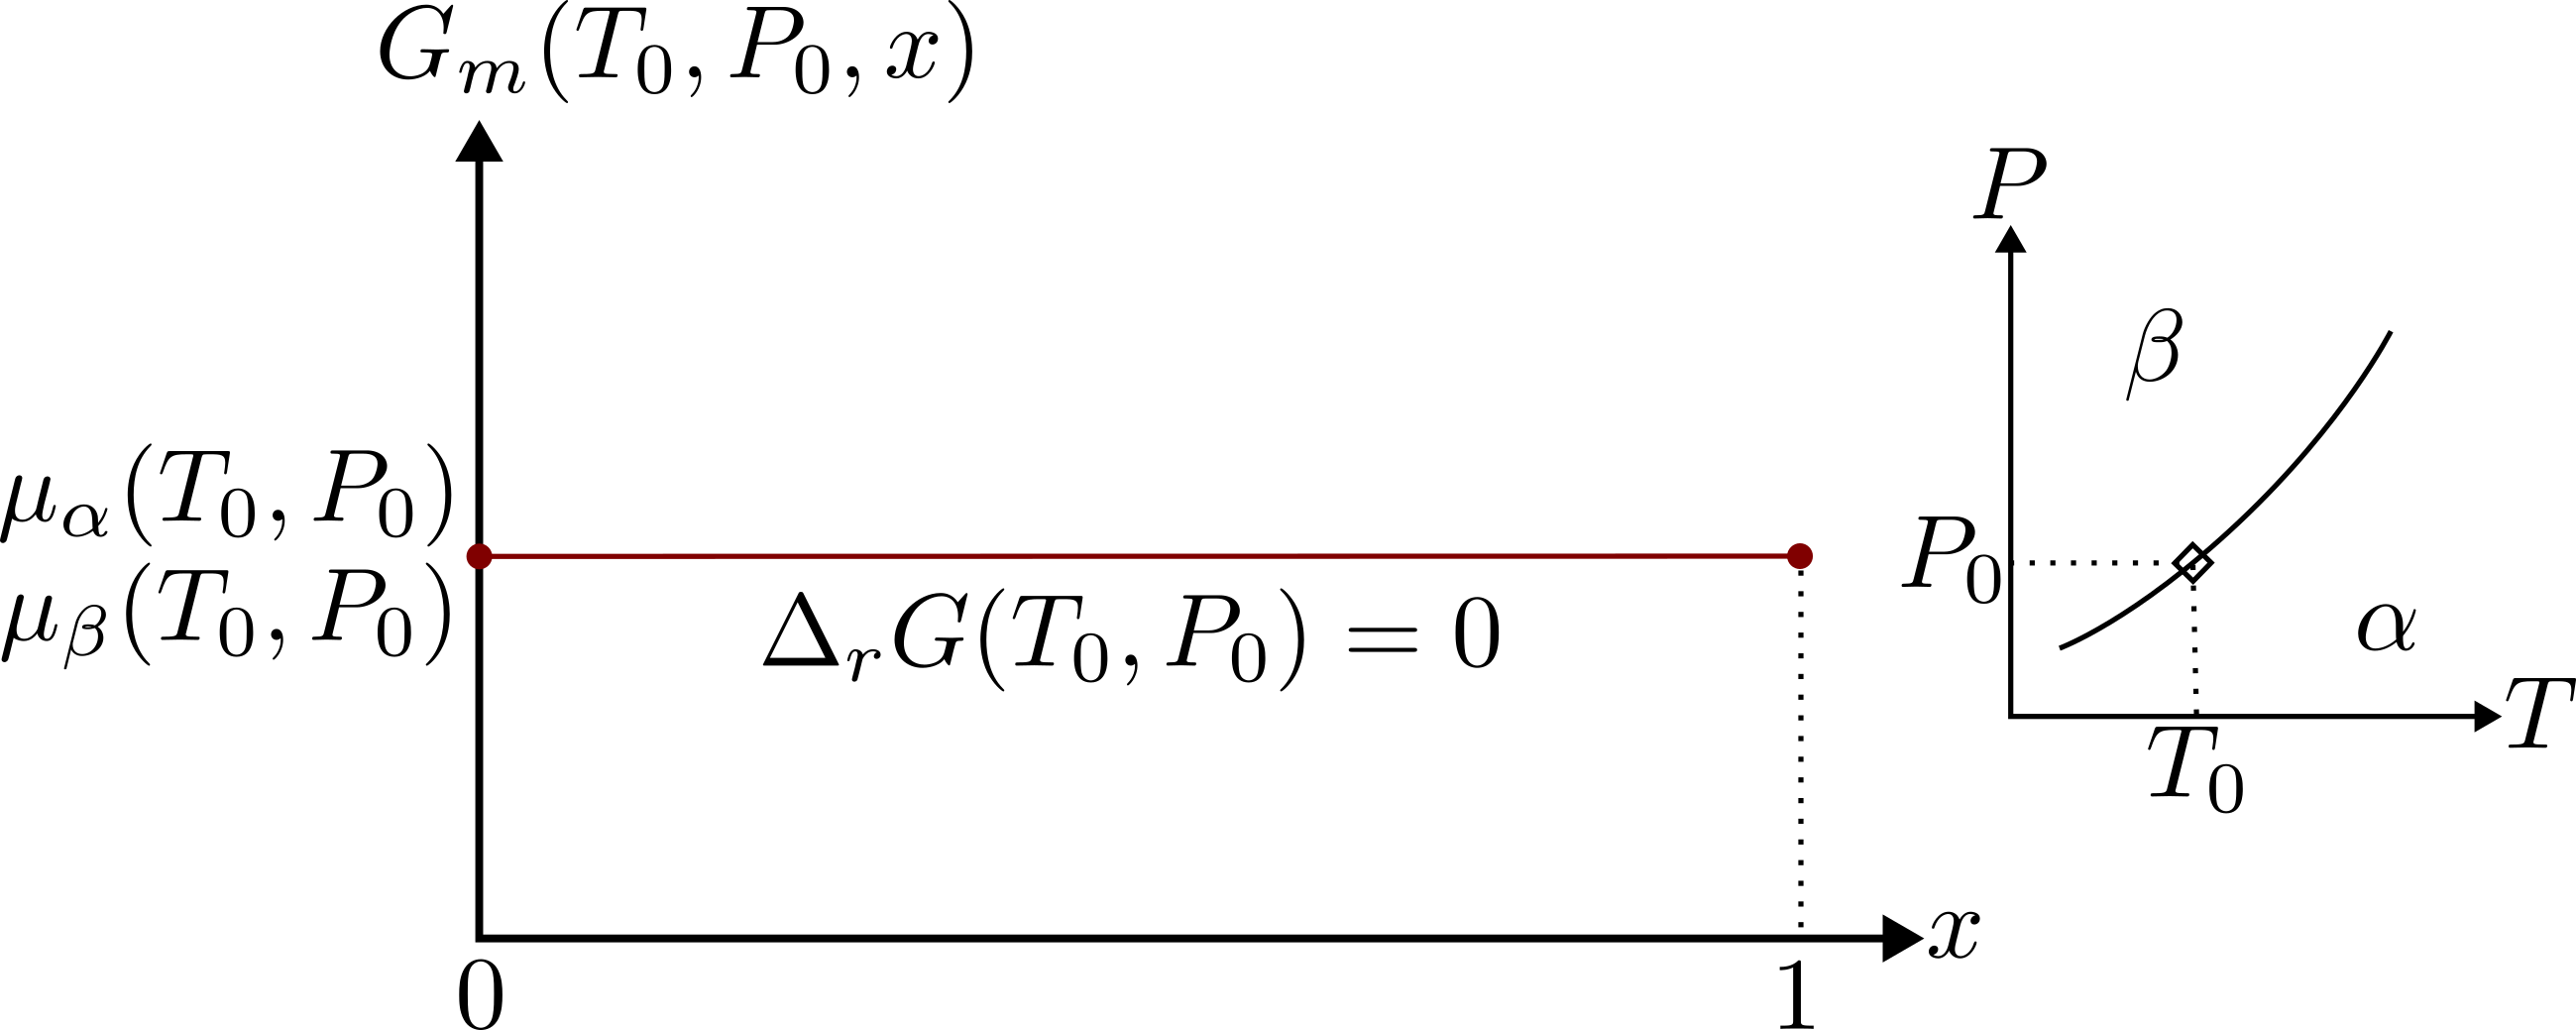
\includegraphics[height=5cm]{../figures/Fig22c}
\captionof{figure}{Allure de $G$ en fonction de la fraction $x$ en phase $\beta$ dans le cas où la phase $\alpha$ est aussi stable que la phase $\beta$. Position correspondante dans le diagramme $(P,T)$}
\end{minipage}
\end{center}

\begin{enumerate}
\item Allure de $G$ en fonction de la fraction $x$ en phase $\beta$ dans le cas où la phase $\beta$ est la plus stable. Position correspondante dans le diagramme $(P,T)$

\item Allure de $G$ en fonction de la fraction $x$ en phase $\beta$ dans le cas où la phase $\alpha$ est la plus stable. Position correspondante dans le diagramme $(P,T)$

\item Allure de $G$ en fonction de la fraction $x$ en phase $\beta$ dans le cas où la phase $\alpha$ est aussi stable que la phase $\beta$. Position correspondante dans le diagramme $(P,T)$
\end{enumerate}


\textbf{Relation avec le diagramme $(T,P)$ :} L'équation de Clapeyron régit l'évolution de la pression et la température lors d'une transition de phase à l'équilibre.
\begin{center}
\begin{minipage}[c]{0.3\colwidth}
\begin{align*}
\frac{dP}{dT} &= \frac{\Delta_r S}{\Delta_r V} = \frac{\Delta_r H}{T \Delta_r V}
\end{align*}
avec :
\begin{align*}
\Delta _r S = S_{m,\beta} - S_{m,\alpha} \\
\Delta _r H = H_{m,\beta} - H_{m,\alpha} \\
\Delta _r V = V_{m,\beta} - V_{m,\alpha}
\end{align*}
\end{minipage}\begin{minipage}[c]{0.3\colwidth}%[t][.12\textwidth]
\begin{tabular}{|C{5cm}|C{5cm}C{5cm}|}
\hline
& $\alpha$ HT & $\alpha$ BT \\
& $S_{m, \alpha} > S_{m, \beta}$ & $S_{m, \alpha} < S_{m, \beta}$ \\
\hline
$\alpha$ HP $V_{m, \alpha} < V_{m, \beta}$ & $\frac{dP}{dT} < 0$ & $\frac{dP}{dT} > 0$  \\
$\alpha$ BP $V_{m, \alpha} > V_{m, \beta}$  & $\frac{dP}{dT} > 0$  & $\frac{dP}{dT} < 0$ \\
\hline
\end{tabular}
\end{minipage}\end{center}

\textbf{Cas de figure}

\begin{center}
\begin{minipage}[t][.07\textwidth][c]{0.48\colwidth}
\centering
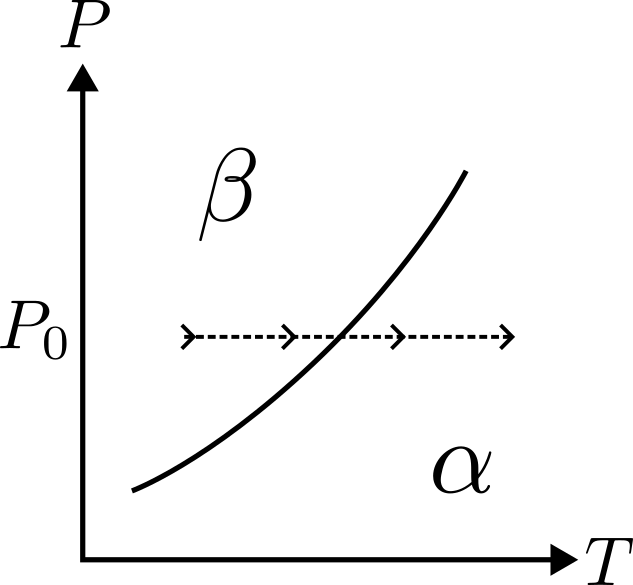
\includegraphics[width=0.3\textwidth]{../figures/Fig23b}
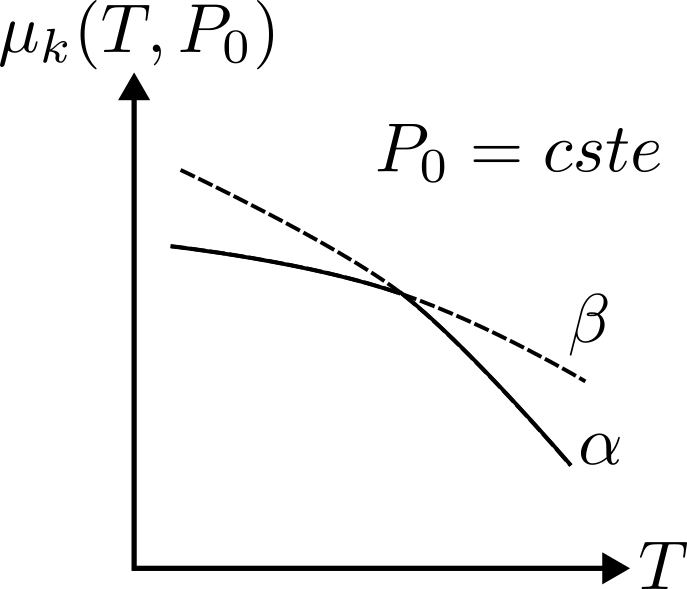
\includegraphics[width=0.3\textwidth]{../figures/Fig23a}
\captionof{figure}{Transition de phase isobare d'une phase $\beta$ basse température vers une phase $\alpha$ haute température : évolution dans le diagramme $(P,T)$ et évolution du potentiel chimique.}
\end{minipage}\begin{minipage}[t][.07\textwidth][c]{0.48\colwidth}
\centering
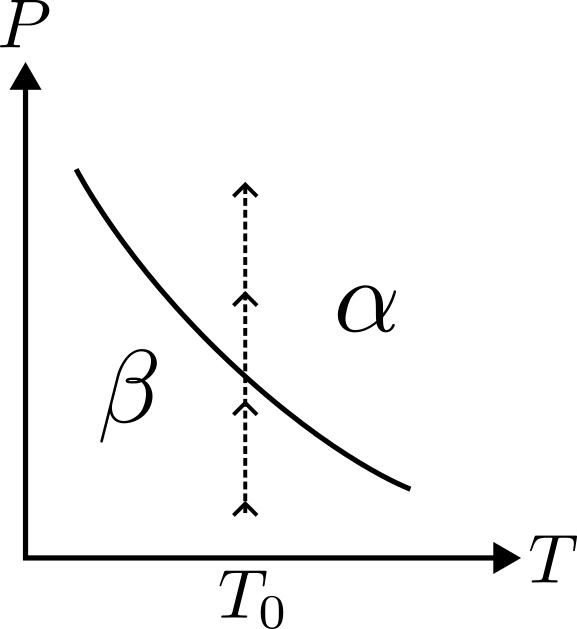
\includegraphics[width=0.3\textwidth]{../figures/Fig23d}
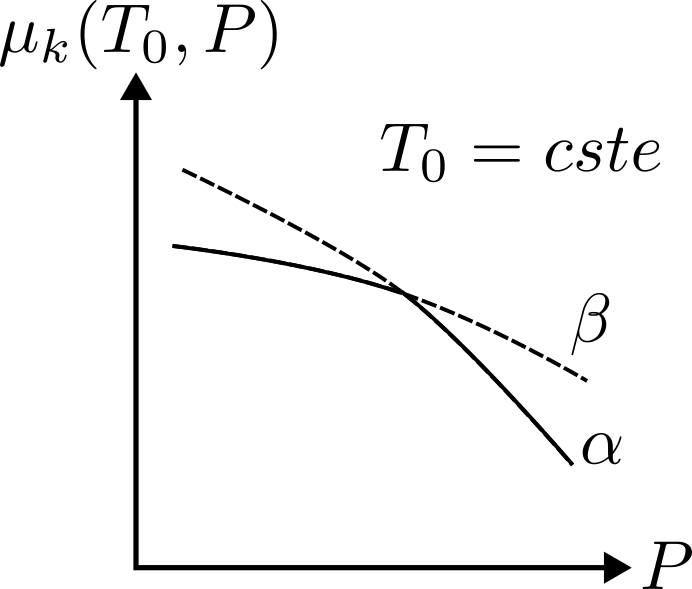
\includegraphics[width=0.3\textwidth]{../figures/Fig23c}
\captionof{figure}{Transition de phase isotherme d'une phase $\beta$ basse pression vers une phase $\alpha$ haute pression : évolution dans le diagramme $(P,T)$ et évolution du potentiel chimique.}
\label{fig:Fe}
\end{minipage}
\end{center}

}


\column{0.25}

\block{Retard à la transition : métastabilité}{

\textbf{Origine de la métastabilité} Dans les transitions de phase, la métastabilité est causée par le coût énergétique qu'il faut payer pour créer une interface entre deux phases.

Pour créer une phase $\beta$ de surface $S$ à partir d'une phase $\alpha$, le travail à fournir par la surface est proportionnel à la surface :
\begin{align*}
W_{\alpha \to \beta} = \gamma_{\alpha / \beta} \cdot S > 0
\end{align*}
où le c{\oe}fficient de proportionnalité positif, noté $\gamma_{\alpha / \beta}$, est appelé au c{\oe}fficient de tension de surface entre la phase $\alpha$/$\beta$ et s'exprime en \si{\joule\per\meter\squared}.

\textbf{\'{E}volution d'une fonction normalisée de l'enthalpie libre en fonction du rayon du cristal.} 

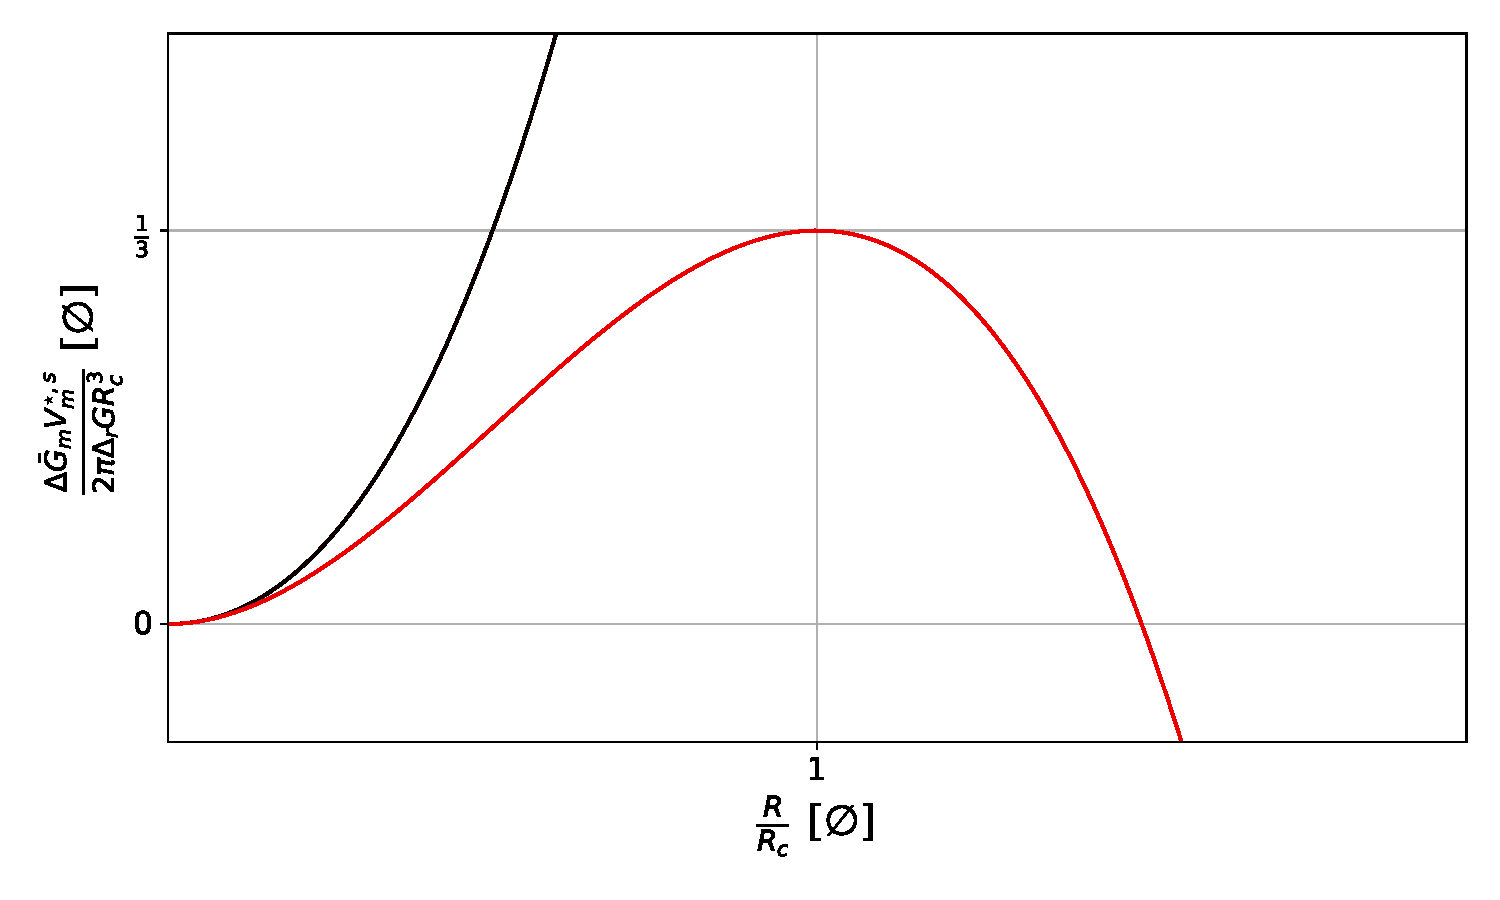
\includegraphics[width=0.9\colwidth]{../figures/Fig24}

\textbf{Condition de cristallisation} Un cristal ne peut apparaître que si son rayon est plus grand qu'un certains rayon critique, noté $R_c$, dont la valeur vaut :
\begin{align*}
R_c = \frac{-2 \gamma_{s/l} V_m^{s, \star}}{\Delta_r G}
\end{align*}
Ce rayon existe (c.-à-d. est positif), si et seulement si l'enthalpie libre de réaction est négative (c.-à-d. que la formation d'un cristal est énergétiquement favorable).

\textbf{Rompre un état de métastabilité} Il faut réaliser une nucléation hétérogène :
\begin{enumerate}
\item en introduisant une fraction de la phase condensée (un grain) permettant de passer au-dessus de la taille critique ;
\item en introduisant une amorce (paroi rugueuse $\ldots$) sur laquelle la phase condensée pourra cristalliser.
\end{enumerate}

}

\end{columns}


\begin{comment}
	\textbf{Coefficients calorifiques} Aussi appelés capacités calorifiques, sont des grandeurs qui permettent de décrire l'évolution de l'énergie du système lors d'une élévation de \SI{1}{\kelvin} de sa température. En général, on regarde cette évolution à volume constant :
\begin{align*}
C_V = \left( \frac{\partial U}{\partial T} \right)_V
\end{align*}
ou à pression constante : 
\begin{align*}
C_p = \left( \frac{\partial H}{\partial T} \right)_P
\end{align*}
Les valeurs tabulées de capacité thermiques le sont généralement de manière intensive en ramenant au nombre de moles ou à la masse du système.
\end{comment}



\end{document}